\documentclass[../mathNotesPreamble]{subfiles}
\begin{document}
\section{JIT 4.4: Shifting up and down}
  $$f(x)  \text{  vs. }f(x)+c$$
    \begin{minipage}{0.5\linewidth}
      \begin{center}
      \begin{tikzpicture}[scale=1.0]
        \begin{axis}[
          axis lines=center,
          axis line style={->},
          xmin=-4, xmax=4.5,
          ymin=-4, ymax=4.5,
          xtick={-4,-3,...,4},
          ytick={-4,-3,...,4},
          ticklabel style={font=\tiny, inner sep=0.75pt},
          xlabel=$x$, xlabel style={at={(ticklabel* cs:1)},anchor=north west},
          ylabel=$y$, ylabel style={at={(ticklabel* cs:1)},anchor=south west},
          legend style={at={(axis cs:2,-1)},anchor=north west},
          every axis plot/.append style={line width=0.95pt}
          ]
          \addplot[domain=-4:4,blue, samples=51, dashed] {x^2};
            \addlegendentry{$x^2$};
          \addplot[domain=-4:4,blue, samples=51] {x^2+2};
            \addlegendentry{$x^2+2$};
          \draw[->, line width = 0.9pt] (axis cs:0.75,9/16)--(axis cs:0.75,40/16);
          \draw[->, line width = 0.9pt] (axis cs:-0.75,9/16)--(axis cs:-0.75,40/16);
        \end{axis}
      \end{tikzpicture}
      \end{center}
    \end{minipage}%
    \begin{minipage}{0.5\linewidth}
      \begin{center}
      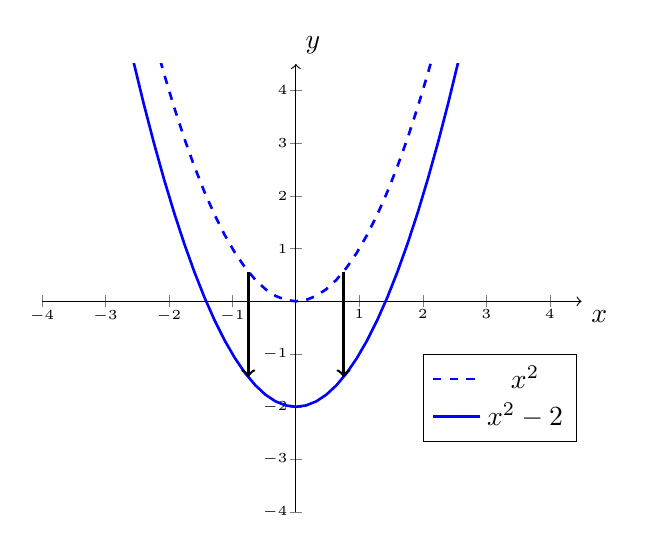
\begin{tikzpicture}[scale=1.0]
        \begin{axis}[
          axis lines=center,
          axis line style={->},
          xmin=-4, xmax=4.5,
          ymin=-4, ymax=4.5,
          xtick={-4,-3,...,4},
          ytick={-4,-3,...,4},
          ticklabel style={font=\tiny, inner sep=0.75pt},
          xlabel=$x$, xlabel style={at={(ticklabel* cs:1)},anchor=north west},
          ylabel=$y$, ylabel style={at={(ticklabel* cs:1)},anchor=south west},
          legend style={at={(axis cs:2,-1)},anchor=north west},
          every axis plot/.append style={line width=0.95pt}
          ]
          \addplot[domain=-4:4,blue, samples=51, dashed] {x^2};
            \addlegendentry{$x^2$};
          \addplot[domain=-4:4,blue, samples=51] {x^2-2};
            \addlegendentry{$x^2-2$};
          \draw[->, line width = 0.9pt] (axis cs:0.75,9/16)--(axis cs:0.75,-23/16);
          \draw[->, line width = 0.9pt] (axis cs:-0.75,9/16)--(axis cs:-0.75,-23/16);
        \end{axis}
      \end{tikzpicture}
      \end{center}
    \end{minipage}
  \vspace*{\stretch{1}}
\end{document}